\newpage
\section{Growing the box}
\genHeader

Ok, back to business. In this SDM, we shall explicitly specify how our learning box is to be built up. We create a specific pattern that will append new
partition elements to the end of a \texttt{Box} that follow our established movement rules (\Cref{fig:membox_depiction}). This means the new partition will
become the \texttt{next} reference of the current last partition, and its \texttt{previous} reference must be connected to the first partition in the box
(\Cref{fig:goal_grow}).

\begin{figure}[htbp]
 	\centering
  	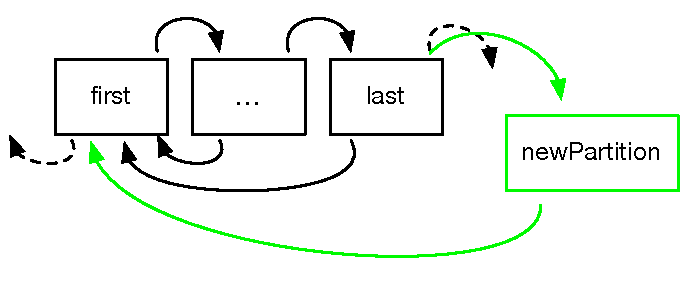
\includegraphics[width=0.7\textwidth]{growBoxNACGoal.pdf}
	\caption{Growing a box by inserting a new partition}
	\label{fig:goal_grow}
\end{figure}
\FloatBarrier

SDMs provide a declarative means of identifying specific partitions via \emph{Negative Application Conditions}, simply referred to as
\mbox{NAC}s.\footnote{Pronounced $\backslash 'nak \backslash$}\define{NAC} \mbox{NAC}s express structures that are forbidden to exist before applying a
transformation rule. In this SDM, the \mbox{NAC} will be an object variable that must not be assigned a value during pattern matching. In the theory of
algebraic graph transformations \cite{EEPT06}, \mbox{NACs} can be arbitrarily complex graphs that are much more general and powerful than what we currently
support in our implementation,\footnote{To be precise, in CodeGen2 from Fujaba} namely only single negative elements (object or link variables).

As depicted in \Cref{fig:goal_grow}, to create an appropriate \mbox{NAC} that constrains possible matches, we'll need to check to see if the currently
matched pattern can be extended to include the negative elements. Suppose the current potential last partition has a \texttt{nextPartition}. This means it
is \emph{not} the absolute last partition, and so the match becomes invalid. We only want to insert a new partition when the \texttt{nextPartition}
of the current potential last partition is null. Similarly, if the current potential first partition has a \texttt{previousPartition}, the match is invalid. The
complete match is therefore made unique through NACs and thus becomes \emph{deterministic} by construction. In other words, if you \emph{grow} the box with this method, there
will always be exactly one first and one last partition of the box.

Of course, to complete this method we still need to determine the size of the new partition. Since the size must be calculated depending on the
rest of the partitions currently in the box (partitions usually get bigger) we'll need to call a helper method, \texttt{determineNextSize} via a
\emph{MethodCallExpression}\define{MethodCallExpression}. As the name suggests, it is designed to access any method defined in \emph{any} class in the current
project.

Due to the algorithmic and non-structural nature of \texttt{determineNextSize}, it will be easier to implement this method via a Java \emph{injection}, rather
than an SDM. We've already declared this method in our metamodel, so its signature will be available for editing in \texttt{BoxImpl.java}.

\begin{stepbystep}

\item Open ``gen/LearningBoxLanguage.impl/BoxImpl.java.'' Scroll to the method declaration, and replace the contents with the code in
\Cref{code:determineNextSize_impl}. Remember not to remove the first comment, which is necessary to indicate that the code is handwritten and needs to be
extracted automatically as an injection. Please do not copy and paste the following code -- the copying process from your pdf viewer to the Eclipse IDE
will likely add invisible characters to the code that eMoflon is unable to handle.

\begin{figure}[htbp]
        \centering
        \begin{lstlisting}[language=Java, keywordstyle={\bfseries\color{purple}}, backgroundcolor=\color{white}]
    public int determineNextSize() {
    	// [user code injected with eMoflon]
        return getContainedPartition().size()*10;
    }
        \end{lstlisting}
        \caption{Implementation of \texttt{removeCard}}
        \label{code:determineNextSize_impl}
\end{figure}


\item Save the file, then right-click on it, either in the package explorer or in the editor window, and choose ``eMoflon/
Create/Update Injection for class'' from the context menu. 

\item Confirm the update in the new \texttt{BoxImpl.inject} file's partial class. \texttt{determineNextSize} is now ready to be used by
your metamodel!

\end{stepbystep}

\newpage
\subsection{Implementing grow}
\visHeader
\hypertarget{growBox vis}{}

\begin{itemize}
 
\item[$\blacktriangleright$] Start by creating the simple story pattern depicted in Fig.~\ref{fig:sdm_grow_1}. This matches the box
(\texttt{this}), with \emph{any} two partitions in the box\footnote{Remember, this is for the \emph{pattern matcher}}.

\begin{figure}[htbp]
\begin{center}
  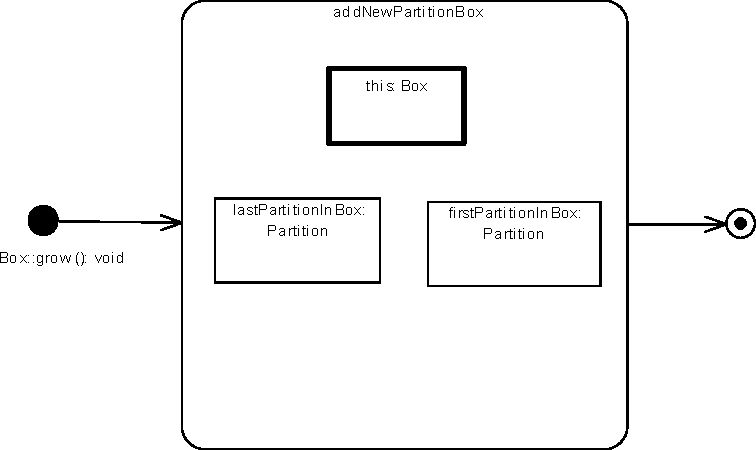
\includegraphics[width=\textwidth]{ea_elementsGrowBox.pdf}
  \caption{Context elements for SDM}  
  \label{fig:sdm_grow_1}
\end{center}
\end{figure}

\item[$\blacktriangleright$] To create the appropriate \mbox{NAC} (to constrain the possible matches for \texttt{lastPartitionInBox}),  create the new object
variable \texttt{nextPartition}, of type \texttt{Partition}, and set \note{Binding Semantics} its \emph{Binding Semantics} to \texttt{negative}
(Fig.~\ref{fig:sdm_grow_2}). The object variable should be visualised as being cancelled or struck out. % why?
 
\begin{figure}[htbp]
\begin{center}
  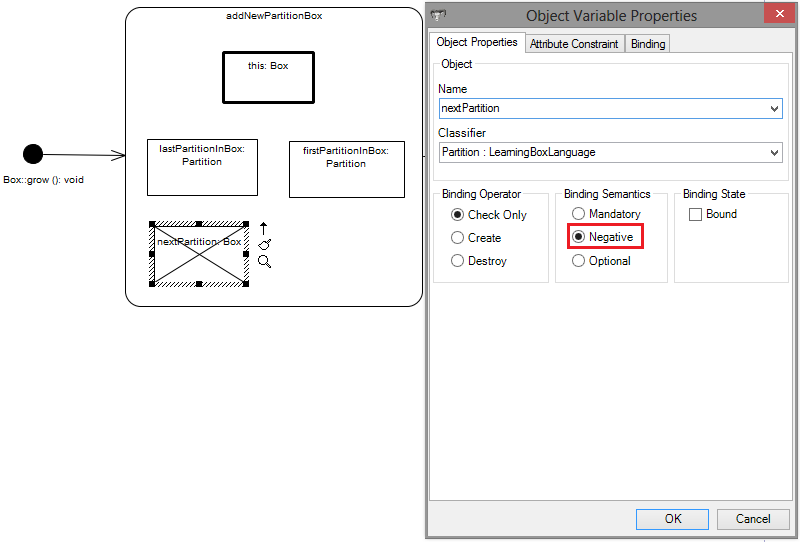
\includegraphics[width=0.9\textwidth]{ea_negElement}
  \caption{Adding a negative element}  
  \label{fig:sdm_grow_2}
\end{center}
\end{figure}
 
\item[$\blacktriangleright$] Now, quick link \texttt{nextPartition} to \texttt{lastPartitionInBox}, but be sure choose the link type carefully! The
\texttt{nextPartition} should play the role of \texttt{next} with respect to \texttt{lastPartitionInBox}.

\item[$\blacktriangleright$] Complete the story pattern so that it closely resembles Fig.~\ref{fig:sdm_grow_3}. 

\begin{figure}[htbp]
\begin{center}
  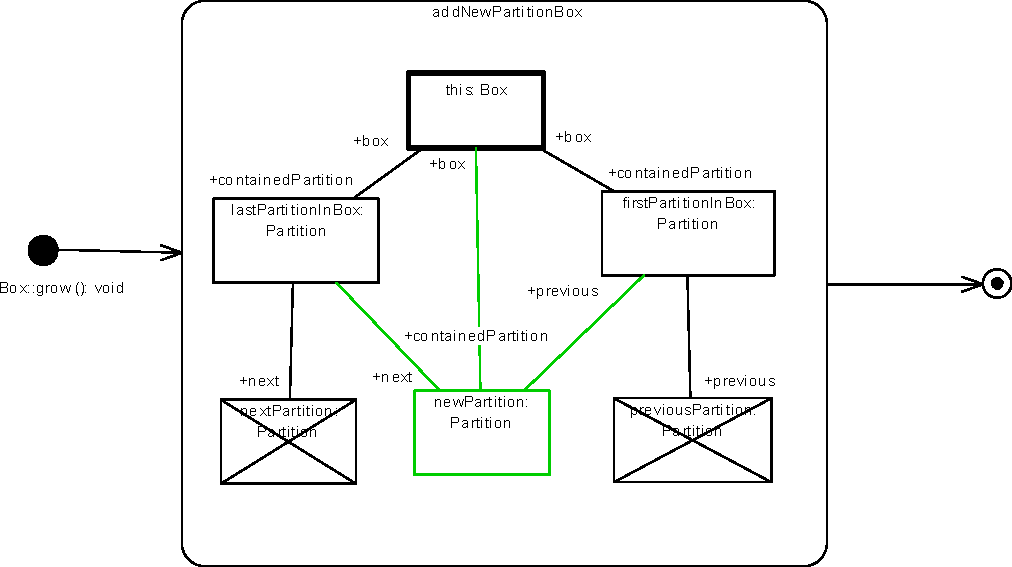
\includegraphics[width=\textwidth]{ea_NACFirstLast.pdf} 
  \caption{Determining the first and last partition with NACs}  
  \label{fig:sdm_grow_3}
\end{center}
\end{figure}
 
\item[$\blacktriangleright$] Notice how the created partition \texttt{newPartition} is `hung' into the box. It becomes the next partition of the current
\emph{last} partition, and has its previous partition set to the first partition in the box (as depicted with the arrows in Fig.~\ref{fig:membox_depiction}).
  
\item[$\blacktriangleright$] To complete this SDM, build the assignment to set the size of the new partition. Go ahead and invoke the corresponding dialogue to
activate the \texttt{:=} operator.

Given that the new size must be calculated using a helper function via a \emph{MethodCallExpression}.\define{MethodCallExpression}A MethodCallExpression is
used to invoke a method defined in any class in the current EA project. Enter the values in Fig.~\ref{fig:sdm_grow_4}, choosing the argument \texttt{this} as
the target, and \texttt{determineNextSize} as the method to be invoked. 

Since \texttt{determineNextSize} doesn't require any parameters, you can ignore the \texttt{Parameters} field this time, but for future reference, parameters
can be specified by choosing the appropriate parameter declaration between guillemets (e.g. \texttt{<Box box>}) found in the drop-down menu and typing in the
value (this is basically a literal expression). Don't forget to press the \texttt{Save} button for every parameter, then \texttt{Add} + \texttt{OK} to confirm
and close the dialogue.
 
 %UPDATE not under 'target' but 'objects'
\begin{figure}[htbp]
\begin{center}
  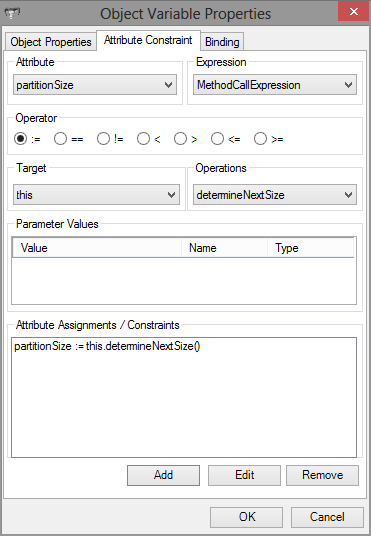
\includegraphics[width=0.5\textwidth]{ea_methodCall.png}
  \caption{Invoking a method via a \texttt{MethodCallExpression} {\bf UPDATE}}  
  \label{fig:sdm_grow_4} 
\end{center}
\end{figure}

\item[$\blacktriangleright$]  If you've done everything right, your SDM should now closely resemble Fig.~\ref{fig:sdm_grow_5}. 

% As usual, try to export, generate code, inspect the
% method implementation and write a JUnit test.  This time around you also have to
% implement the helper method \texttt{determineNextSize} directly in the
% generated code
% (\texttt{gen/\-LearningBoxLanguage/\-facade/\-impl/\-LearningBoxUtilImpl}).
% Don't forget to add \texttt{@generated NOT} to the Java doc comment of the
% method so the code generator preserves your code in future runs.
% When testing (which you will \emph{of course} do right?), note that you can only grow a ``minimal'' box that has at least a first and last partition, i.e., a box with 
%no partitions at all cannot be grown using our specified SDM. 

\begin{figure}[htbp]
\begin{center}
  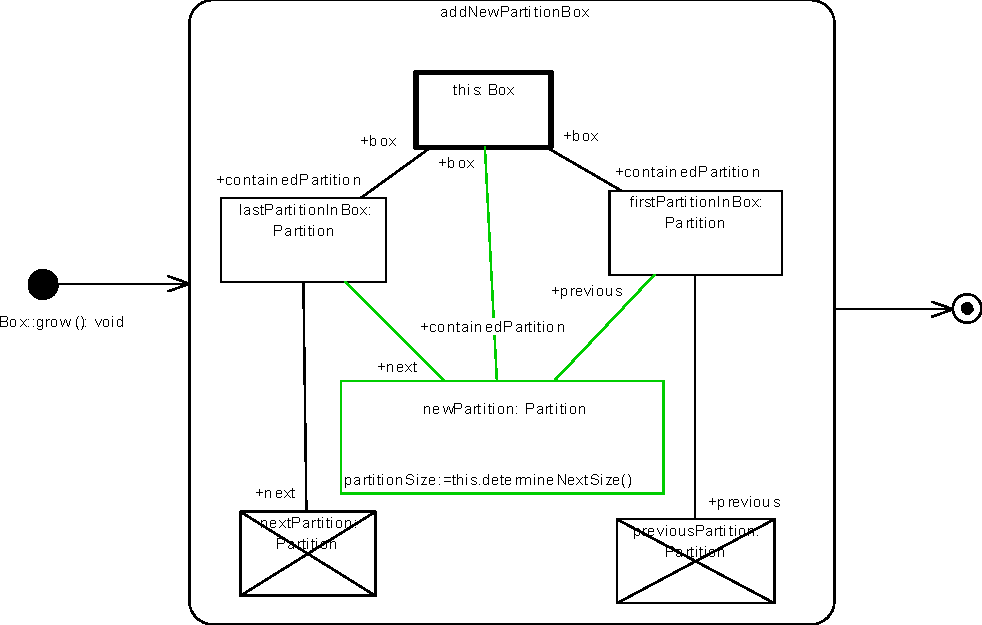
\includegraphics[width=0.9\textwidth]{ea_completeActivityGrowBox.pdf}
  \caption{Complete SDM for \texttt{Box::grow}}  
  \label{fig:sdm_grow_5}
\end{center}
\end{figure}

\item[$\blacktriangleright$]  That's it - your \texttt{grow} SDM is complete! This was probably the most challenging SDM to build, so give yourself a solid 
pat on the back. If you found it easy then \ldots gee whiz, I don't think i'm doing my job correctly. To see how this is done in the texual syntax, review
Fig.~\ref{fig:patternComplete}.\footnote{We do recommend reading the instructions for this one, however, since NACs can be tricky.}

\end{itemize}

